\documentclass[11pt]{article}
\usepackage[a4paper,margin=1in]{geometry}
\usepackage{amsmath,amssymb,amsthm}
\usepackage{graphicx}
\usepackage[hidelinks]{hyperref}

\newtheorem{theorem}{Theorem}
\newtheorem{corollary}{Corollary}
\newtheorem{remark}{Remark}

\DeclareMathOperator{\Lip}{Lip}

\title{Absolute-Sum Stability for the Real Lipschitz Numerical Index Question}
\author{Automatic math-discovery packet}
\date{June 13, 2026}

\begin{document}
\maketitle

\section*{Source question}

The source paper is Antonio Perez-Hernandez,
\emph{Lipschitz vs Linear Numerical Index in certain Banach spaces},
arXiv:2507.18208. It studies the question, originally posed by
Wang--Huang--Tan, whether the Lipschitz numerical index \(n_L(X)\) and the
classical numerical index \(n(X)\) always coincide.

\begin{figure}[h]
\centering
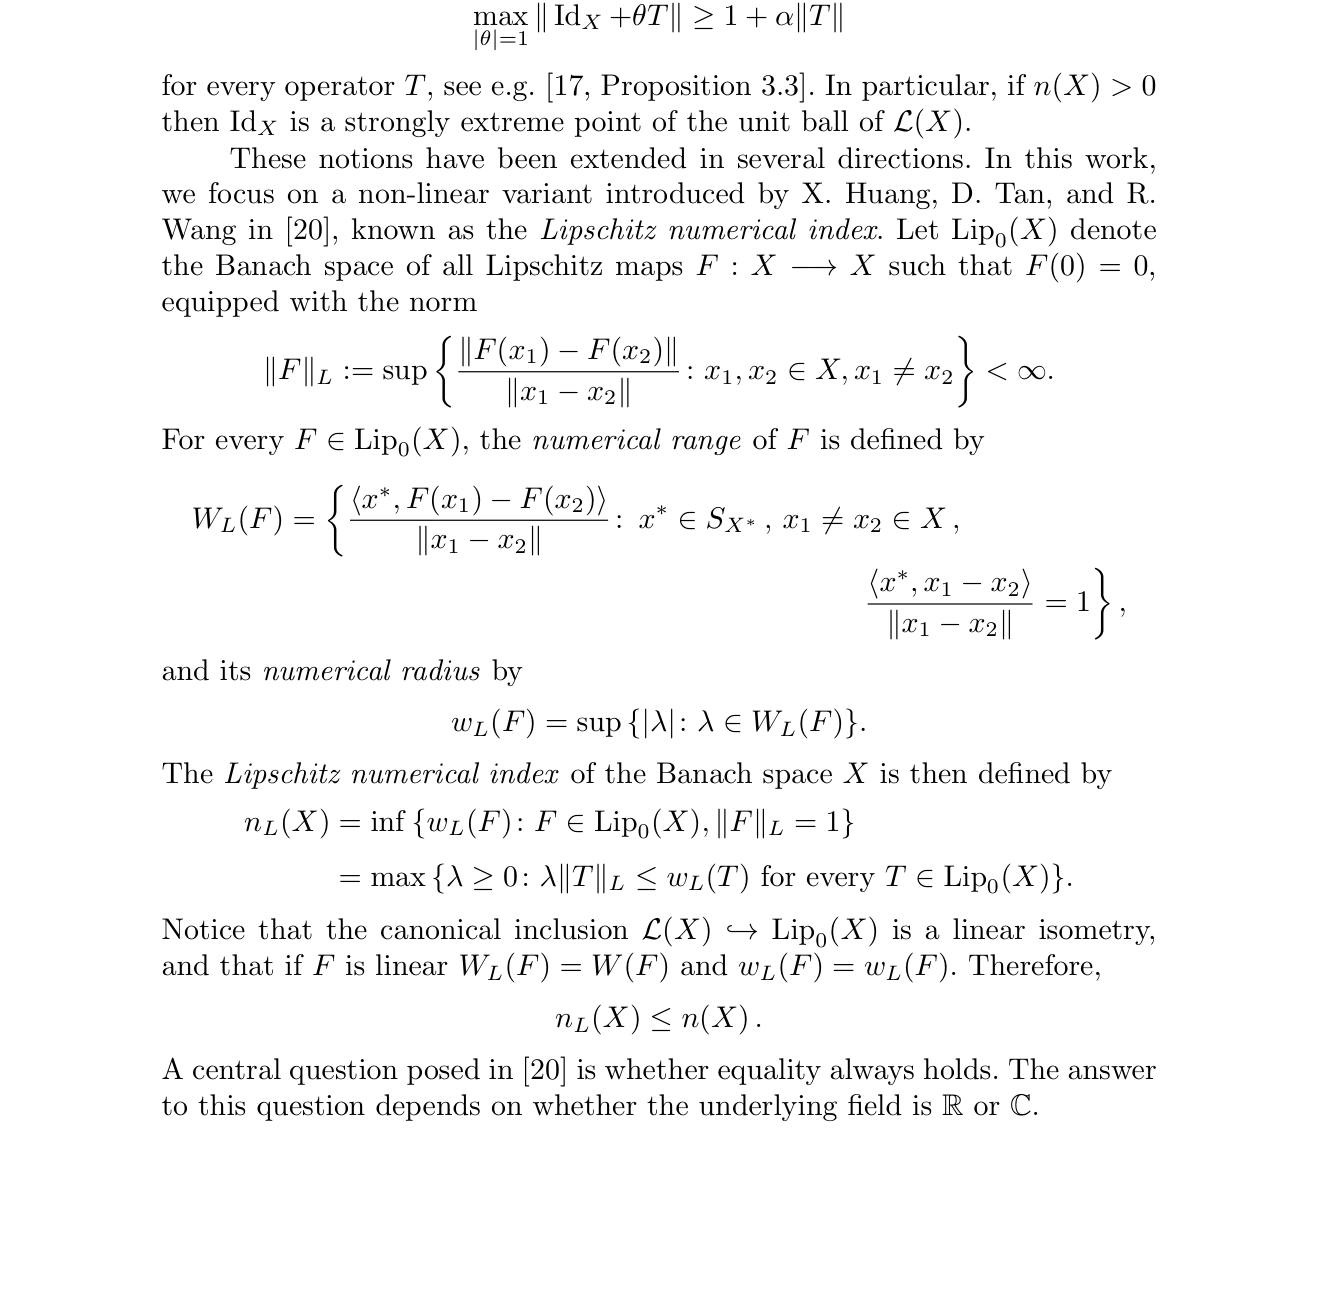
\includegraphics[width=\textwidth]{figures/open_question_page2_crop.png}
\caption{The paper defines the Lipschitz numerical index and records the central equality question.}
\end{figure}

\begin{figure}[h]
\centering
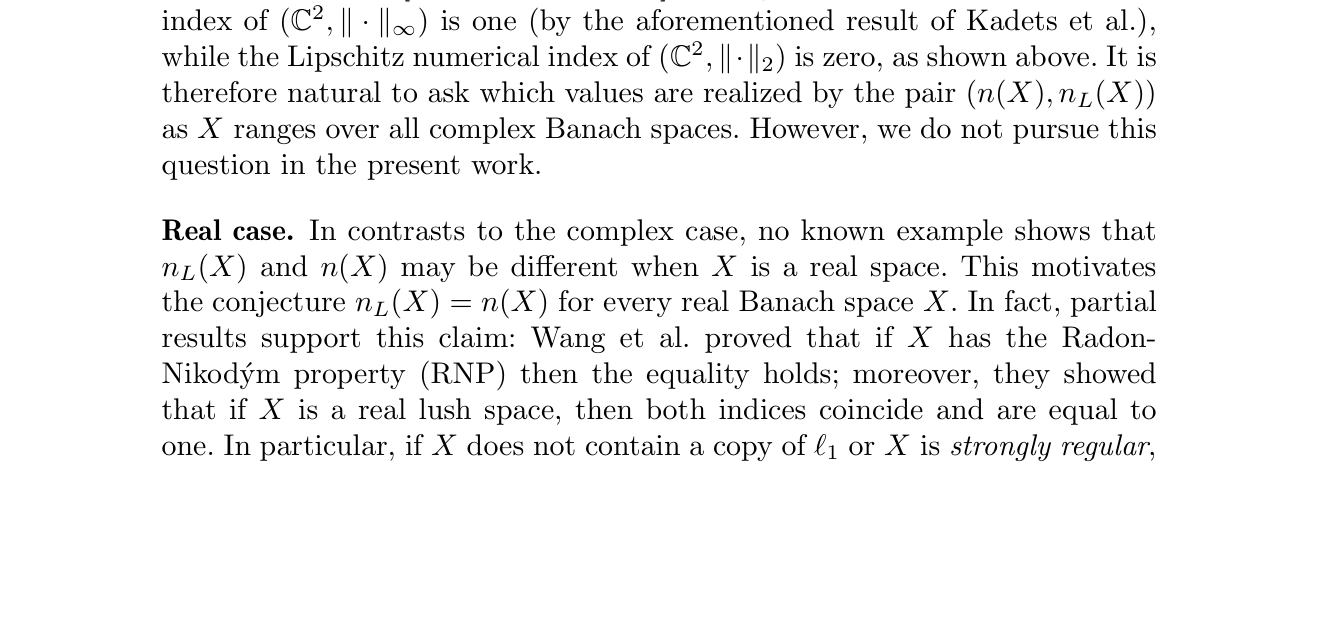
\includegraphics[width=\textwidth]{figures/real_case_conjecture_page3_crop.png}
\caption{In the real case the source states the conjectural equality \(n_L(X)=n(X)\) for every real Banach space.}
\end{figure}

\begin{figure}[h]
\centering
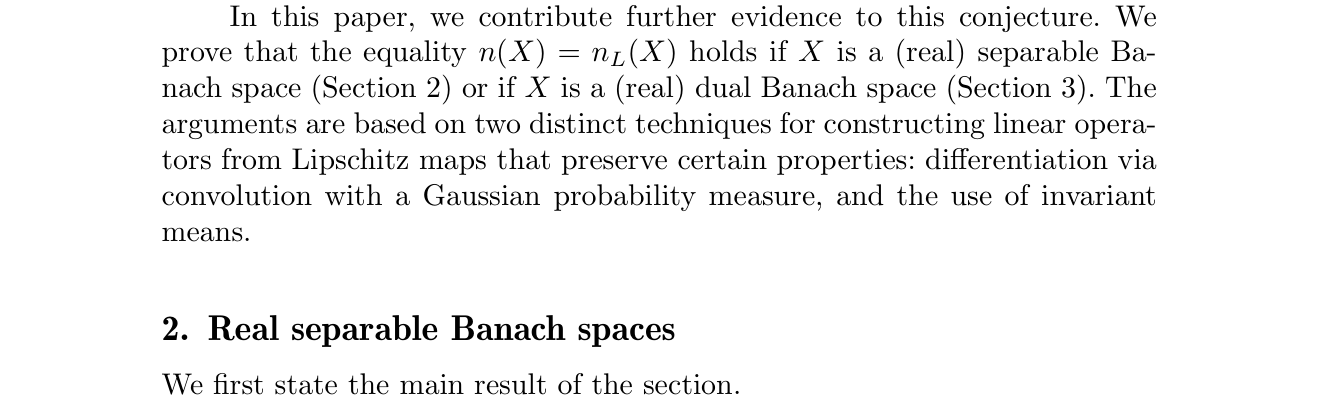
\includegraphics[width=\textwidth]{figures/separable_theorem_page4_crop.png}
\caption{The source paper proves the equality for real separable Banach spaces. It also proves it for real dual Banach spaces.}
\end{figure}

\clearpage

\section*{Definitions and external inputs}

For a Banach space \(X\), write \(\Lip_0(X)\) for the Banach space of
Lipschitz maps \(F:X\to X\) with \(F(0)=0\), equipped with the Lipschitz norm
\[
  \|F\|_L=\sup_{x\ne y}\frac{\|F(x)-F(y)\|}{\|x-y\|}.
\]
The Lipschitz numerical radius is denoted \(w_L(F)\), and
\[
  n_L(X)=\inf\{w_L(F):F\in \Lip_0(X),\ \|F\|_L=1\}.
\]
For linear operators, \(w_L\) agrees with the classical numerical radius
\(w\), hence always \(n_L(X)\leq n(X)\).

We use the following published inputs.

\begin{enumerate}
\item Perez-Hernandez proves that \(n_L(Y)=n(Y)\) for every real separable
Banach space \(Y\), and also for every real dual Banach space \(Y\).
\item Wang--Huang--Tan prove that if
\[
  X=\left(\bigoplus_{\gamma\in\Gamma}X_\gamma\right)_{c_0},\qquad
  X=\left(\bigoplus_{\gamma\in\Gamma}X_\gamma\right)_{\ell_1},
  \quad\text{or}\quad
  X=\left(\bigoplus_{\gamma\in\Gamma}X_\gamma\right)_{\ell_\infty},
\]
then
\[
  n_L(X)=\inf_{\gamma\in\Gamma} n_L(X_\gamma).
\]
\item The corresponding classical numerical-index formula is
\[
  n(X)=\inf_{\gamma\in\Gamma} n(X_\gamma)
\]
for the same three sums. This formula is classical; it is also recorded in
the absolute-sum literature of Martin--Meri--Popov--Randrianantoanina.
\end{enumerate}

\section*{Claim}

\begin{theorem}
Let \(\{X_\gamma:\gamma\in\Gamma\}\) be a family of real Banach spaces such
that
\[
  n_L(X_\gamma)=n(X_\gamma)
  \qquad(\gamma\in\Gamma).
\]
Let \(X\) be one of the three sums
\[
  \left(\bigoplus_{\gamma\in\Gamma}X_\gamma\right)_{c_0},\qquad
  \left(\bigoplus_{\gamma\in\Gamma}X_\gamma\right)_{\ell_1},\qquad
  \left(\bigoplus_{\gamma\in\Gamma}X_\gamma\right)_{\ell_\infty}.
\]
Then
\[
  n_L(X)=n(X).
\]
\end{theorem}

\begin{proof}
By the Wang--Huang--Tan stability theorem for the Lipschitz numerical index,
\[
  n_L(X)=\inf_{\gamma\in\Gamma} n_L(X_\gamma).
\]
By the hypothesis on the summands this is
\[
  \inf_{\gamma\in\Gamma} n(X_\gamma).
\]
Finally, the classical stability formula for the numerical index of
\(c_0\)-, \(\ell_1\)-, and \(\ell_\infty\)-sums gives
\[
  \inf_{\gamma\in\Gamma} n(X_\gamma)=n(X).
\]
Therefore \(n_L(X)=n(X)\).
\end{proof}

\begin{corollary}
If each \(X_\gamma\) is either a real separable Banach space or a real dual
Banach space, then the three sums above satisfy \(n_L(X)=n(X)\).
\end{corollary}

\begin{proof}
Perez-Hernandez proves \(n_L(Y)=n(Y)\) for every real separable Banach space
and for every real dual Banach space. Apply the theorem to the family
\(\{X_\gamma\}\).
\end{proof}

\section*{Relation to previous run work}

The earlier packet
\[
\texttt{solutions/partial/2507.18208\_c0\_sum\_lipschitz\_numerical\_index/}
\]
proved the special case of \(c_0\)-sums of separable real spaces by a direct
countable-coordinate reduction. The present packet gives a broader but more
literature-driven partial result: it also covers \(\ell_1\)- and
\(\ell_\infty\)-sums and any summand class for which the equality is known,
including real dual spaces.

\section*{A route not promoted}

A more ambitious separable-projection reduction was tested. Suppose every
separable subset of a real Banach space \(X\) is contained in a separable
range \(E\) of a norm-one projection \(P:X\to E\). Given a norm-one
Lipschitz map \(F:X\to X\), one can choose \(E\) containing a near
Lipschitz-norm-attaining pair \(x,y\) and the two values \(F(x),F(y)\). Then
the compressed map \(G=P F|_E:E\to E\) satisfies \(\|G\|_L\) almost \(1\) and
\[
  w_L(G)\leq w_L(F).
\]
Since \(E\) is separable, Perez-Hernandez gives
\[
  w_L(F)\geq w_L(G)\geq n(E)\|G\|_L.
\]
However, this does not imply \(w_L(F)\geq n(X)\) unless one also knows the
classical comparison \(n(E)\geq n(X)\). That comparison is available for the
coordinate summands in the three absolute sums used above, but it is not a
consequence of arbitrary one-complementability alone. For that reason, the
projectional-skeleton route is recorded only as an attempt, not as a theorem.

\section*{Literature and novelty check}

Searches were made for the source arXiv id, the phrases
\emph{Lipschitz numerical index}, \emph{projectional skeleton},
\emph{one-complemented}, and \emph{separable complementation}, together with
the exact equality \(n_L(X)=n(X)\). The relevant hits were the source paper,
Wang--Huang--Tan's 2014 stability paper, Choi--Jung--Tag's 2025 paper on
one-complemented increasing unions, and the classical absolute-sum paper of
Martin--Meri--Popov--Randrianantoanina. No later paper was found explicitly
stating the corollary above as a partial answer to the 2025 real-case
question.

\section*{Verification notes}

This packet is a theorem-by-combination. The proof is complete if the two
stability formulas are accepted as external inputs. The human verifier should
focus on:
\begin{itemize}
\item confirming that Wang--Huang--Tan's formula applies to arbitrary
families under the \(c_0\), \(\ell_1\), and \(\ell_\infty\) norms;
\item confirming the matching classical numerical-index formula for the same
three sums;
\item checking that the packet is understood as a partial result and not a
solution for arbitrary real Banach spaces.
\end{itemize}

\begin{thebibliography}{9}

\bibitem{Perez}
A. Perez-Hernandez,
\emph{Lipschitz vs Linear Numerical Index in certain Banach spaces},
arXiv:2507.18208.

\bibitem{WHT}
R. Wang, X. Huang, and D. Tan,
\emph{On the numerical radius of Lipschitz operators in Banach spaces},
J. Math. Anal. Appl. 411 (2014), 1--18; arXiv:1211.5753.

\bibitem{MMPR}
M. Martin, J. Meri, M. Popov, and B. Randrianantoanina,
\emph{Numerical index of absolute sums of Banach spaces},
J. Math. Anal. Appl. 375 (2011), 207--222; arXiv:1003.3269.

\bibitem{CJT}
G. Choi, M. Jung, and H.-J. Tag,
\emph{On the Lipschitz numerical index of Banach spaces},
Collect. Math. 76 (2025), 81--103; arXiv:2110.13821.

\end{thebibliography}

\end{document}
